\subsubsection{Incremento 8}
\textit{\textbf{Periodo}: dal 2021-03-26 al 2021-03-31}

\myparagraph{Obiettivi}
Gli obiettivi definiti per questo incremento sono i seguenti:
\begin{itemize}
\item implementazione acquisto prodotti, compreso di gestione del carrello e checkout;
\item incremento della documentazione.
\end{itemize}

\myparagraph{Attività}
Per raggiungere gli obiettivi, vengono svolte le seguenti attività:
\begin{itemize}

\item \textbf{codifica e progettazione}:
\begin{itemize}
\item implementazione UC6 - Visualizzazione prodotti nel carrello;
\item implementazione UC7 - Rimozione prodotto nel carrello;
\item implementazione UC8 - Modifica quantità di un prodotto nel carrello;
\item implementazione UC9 -  Visualizzazione costo totale e tasse applicate;
\item implementazione UC10 - Acquisto prodotti;
\item implementazione UC11 - Visualizzazione riepilogo ordine;
\item implementazione UC14 - Visualizzazione ordini effettuati dall’utente;
\item implementazione UC20 - Inserimento nel carrello dei prodotti selezionati;
\item implementazione UC24 - Modifica della quantità selezionata del prodotto;
\item implementazione UC25 - Inserimento nel carrello del prodotto visualizzato;
\item implementazione UC34 -  Visualizzazione lista ordini;
\item creazione diagrammi UML inerenti.

\end{itemize}

\item \textbf{ampliamento documentazione e verifiche}:
\begin{itemize}
\item incremento del \textit{\MU{}} per i casi d'uso implementati;
\item incremento del \textit{\MM{}} per i casi d'uso implementati;
\item incremento dell'\textit{Allegato tecnico}\ped{G} per i casi d'uso implementati;
\item incremento del \Glossariov{2.0.0};
\item rilevazione e registrazione di metriche, esiti di verifica e obiettivi di qualità;
\item aggiornamento dei rischi rilevati;
\item calcolo e registrazione del consuntivo di periodo.
\end{itemize}

\end{itemize}
\myparagraph{Diagramma di Gantt}
\begin{figure}[H]
\centering

\centerline{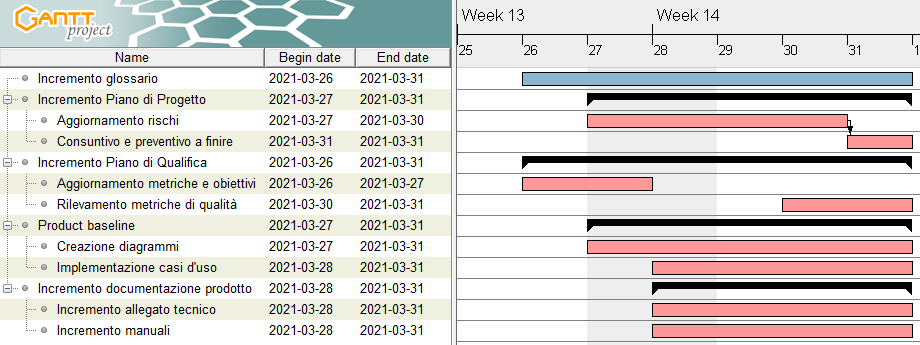
\includegraphics[scale=0.6]{res/Pianificazione/Fasi/CodificaIncrementi/ganttIncremento8}}
\caption{Diagramma di Gantt per l'incremento 8}
\end{figure}